\documentclass[00_mcda_tutorial.tex]{subfiles}

\begin{document}
\begin{sidebar*}

\section*{Tutorial 6: Survey creation and response analysis (Enterprise edition)}
\addtocounter{section}{1}
\addcontentsline{toc}{section}{\protect\numberline{}Tutorial 6: survey creation and response analysis}

\subsection*{Subjects covered}
\begin{itemize}
  \item Creating a survey
  \item Customising and publishing a survey
  \item Analysing survey responses
\end{itemize}

\subsection*{Prerequisites}
\noindent This tutorial assumes some familiarity with the ADDIS/MCDA interface, either from following previous tutorials or independent study.

\subsection*{ADDIS MCDA surveys}
\noindent ADDIS/MCDA can be used to elicit personal preferences and explore their consequences for the benefit/risk balance of a given problem.
However, in many situations one might be more interested in the preferences of a larger group of people, e.g. a group of regulators or the patient population for a disease.
ADDIS/MCDA lets you create and distribute surveys to such groups simply by sharing a hyperlink.
Users following this link will have their preferences elicited, and their response will be made available for aggregate-level analysis.
This tutorial guides you through the process of creating and publishing a survey, as well as the subsequent analysis of survey responses.

\subsection*{Getting started}
\noindent \leftpointright \, Open your browser and navigate to your MCDA server, and sign in.
\newline

\noindent \leftpointright \, Create a new workspace for the tutorial by clicking the ‘Create workspace’ button and choosing the ‘Lixisenatide simplified’ option from the tutorial workspaces.
\newline

\subsection*{Creating the survey}
\noindent \leftpointright \, Navigate to the 'Problem definition' tab.  Note that the 'Create survey' button is disabled. Hovering your mouse over the button will inform you that there are missing or empty values in your problem table, which you can verify in the effects table shown. Since it would be redundant to create surveys based on problems which cannot be analysed, this is not possible in the system.
\newline

\noindent \leftpointright \, Create a new subproblem called 'For survey' without empty cells and with only a single data source per criterion. We recommend deselecting Exenatide, and using the pooled data source for this example, as in Figure~\ref{fig:survey_problem}.
\newline

{	
	\centering
	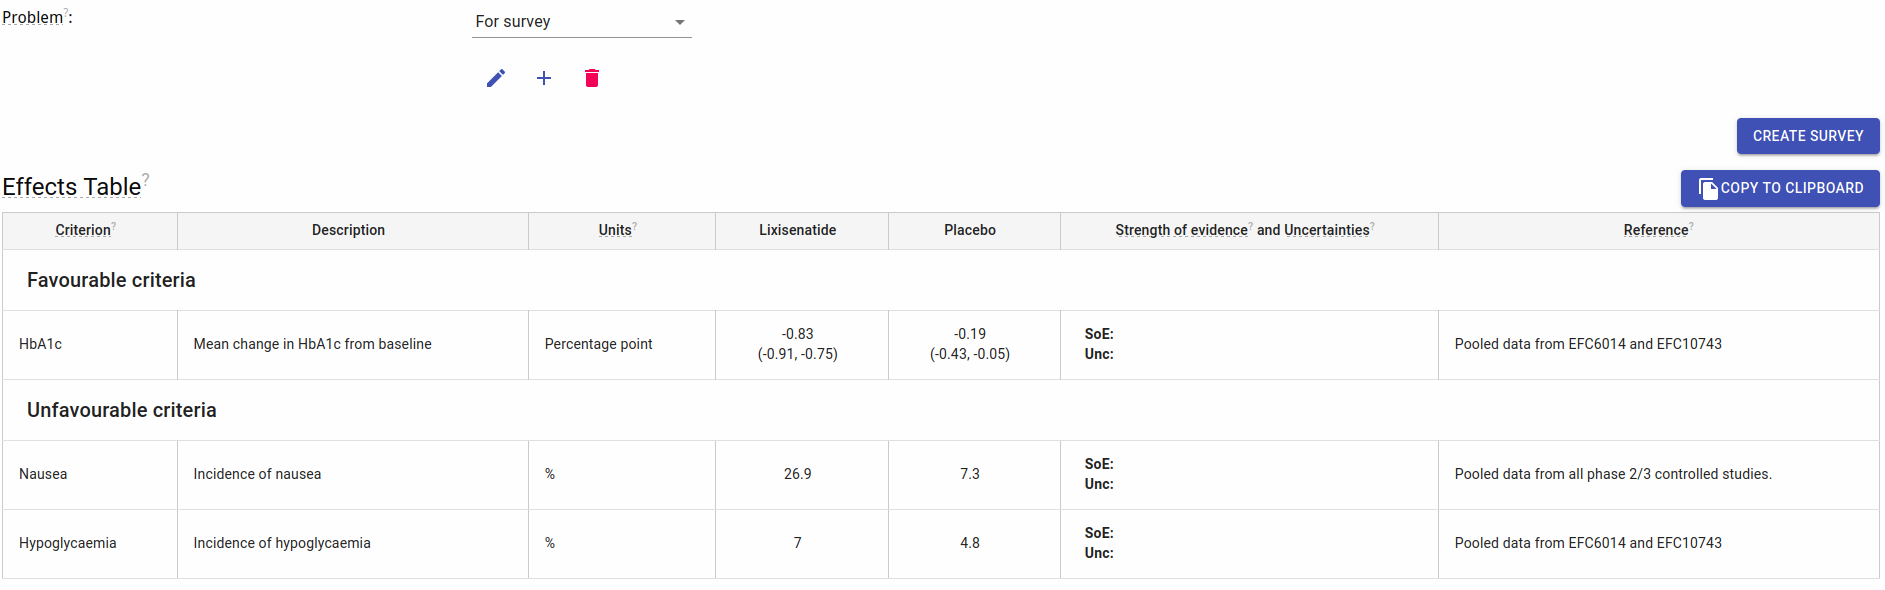
\includegraphics[width=\textwidth]{fig/surveyProblem.png}
	\captionof{figure}{Simplified effects table for lixisenatide, ready to be used as basis for a survey.}
	\label{fig:survey_problem}
	\par
}

\noindent \leftpointright \, Note that the 'Create survey' button is now enabled. Click it, take a moment to read the question and click 'Yes'. The dialog will close and you will be redirected to the newly created survey.
\newline

\noindent \faLightbulbO \, For simplicity's sake, each problem in ADDIS/MCDA can currently have precisely one survey based on it. Should you want to create multiple surveys based on the same problem table for any reason, create a new problem from the base problem and create a new survey for the new problem.

\subsection*{Modifying and publishing the survey}

\noindent \leftpointright \, Take a look at your new survey. Note that the ADDIS/MCDA survey tool is separated into tabs, which are intended to guide you through the process of editing and publishing the study, progressing from left to right. The first ('Problem') tab shows you the effects table of the problem it is based on, and the scale ranges and units of the effects (Figure~\ref{fig:survey_welcome}).
\newline

{	
	\centering
	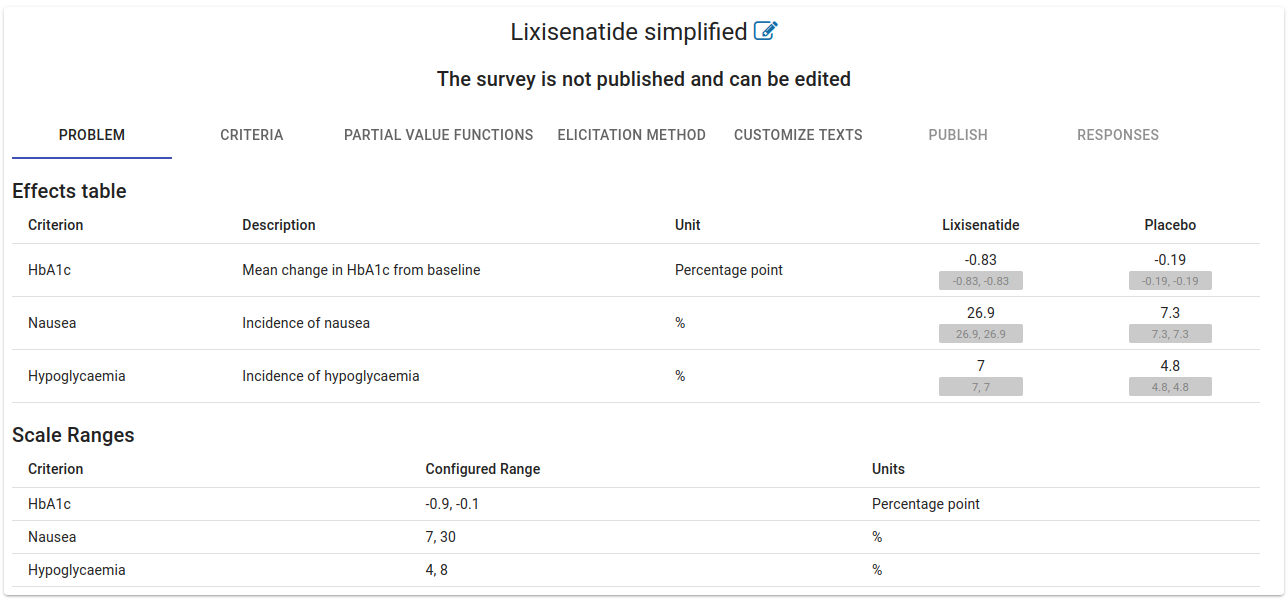
\includegraphics[width=\textwidth]{fig/surveyWelcome.png}
	\captionof{figure}{Welcome screen of the survey tool, showing the effects table the survey is based on.}
	\label{fig:survey_welcome}
	\par
}


\noindent \leftpointright \, Click on the 'Criteria' tab. Here you can edit the name, description and unit of measurement for the criteria. If your survey is intended for laypeople you might for example want to edit 'HbA1c' to be called 'Blood sugar level change.'
\newline

\noindent \faExclamationTriangle \, Editing the unit of measurement here is purely cosmetic and will not affect any functionality besides labelling. It is your responsibility to not e.g. give a criterion the unit '\%' which reports non-percentage values.
\newline

\noindent \leftpointright \, Click on the 'Partial value functions' tab. Here you set the direction of the partial value functions for the criteria, i.e. whether lower values are better than higher ones or vice versa. In this example, we wish for lower blood sugar levels as well as fewer incidences of nausea and hypoglycemia, so all partial value functions should be set to 'lower.'
\newline

\noindent \faLightbulbO \, The main ADDIS/MCDA application lets you define more complex non-linear partial-value functions, but we have omitted this option here for simplicity's sake.
\newline

\noindent \leftpointright \, Click on the 'Elicitation Method' tab. Here you choose the method that will be used to elicit the responders' preferences. The same options are supported here as in the main ADDIS/MCDA application. For most users we recommend the 'Choice based matching' method which asks a series of questions requiring the responder to choose between scenarios. For this tutorial however, please select the 'Matching' option.
\newline

\noindent \leftpointright \, Adjust the test slider for one of the criteria, then change the step size and adjust the slider again. Note the difference in behaviour. During matching, the surveyee will be asked to adjust a value so that two alternative scenarios are equivalent. Setting the step size here will determine the minimum adjustment size they can make. Choose a step size for each criterion that feels appropriate to you given the scale range (meaning the range of possible values for that criterion).
\newline

\noindent \leftpointright \, Click on the 'Customize texts' tab. Here you can customise several of the texts that will be shown to the responders during the survey. Note that the 'Default' button in each text editor will always return the text to the simple defaults first shown here.
\newline

\noindent \faLightbulbO \, The 'Question during matching elicitation' text has several phrases in all capitals. These are template values, which will be substituted by the appropriate text or value during the survey. These templates are covered in more detail in the following 'test run' section of this tutorial. Several other elicitation methods also let you use templates in the accompanying texts.
\newline

\noindent \leftpointright \, Make any preliminary text changes that you wish, and then click the 'Test run' button. This will let you run through a demonstration of what a responder will encounter during your survey. Note the two round buttons at the bottom, which allow you to edit texts in place and stop the test run, respectively (Fig.~\ref{fig:survey_edit_controls}).
\newline

{	
	\centering
	
\includegraphics[width=.3\textwidth]{fig/surveyEditControls.png}
	\captionof{figure}{Edit text (left) and stop test run (right) buttons.}
	\label{fig:survey_edit_controls}
	\par
}

\noindent \leftpointright \, On the welcome screen in the test run, click the edit button (pencil icon). A dialog will open similar to the one on the Customize texts tab. Note that the criteria names have been replaced by so-called template texts, surrounded by '\%' symbols. Click the question mark button in the editor's toolbar to the right of the 'Default' button to show a legend with the available template texts. Use this knowledge to extend the question with information about the current worst value, e.g. 'It is currently X' where X is the worst value of criterion 1. Click the 'Save' button and note the effect of this change. See Fig.~\ref{fig:templateEditing}
\newline

{	
	\centering
	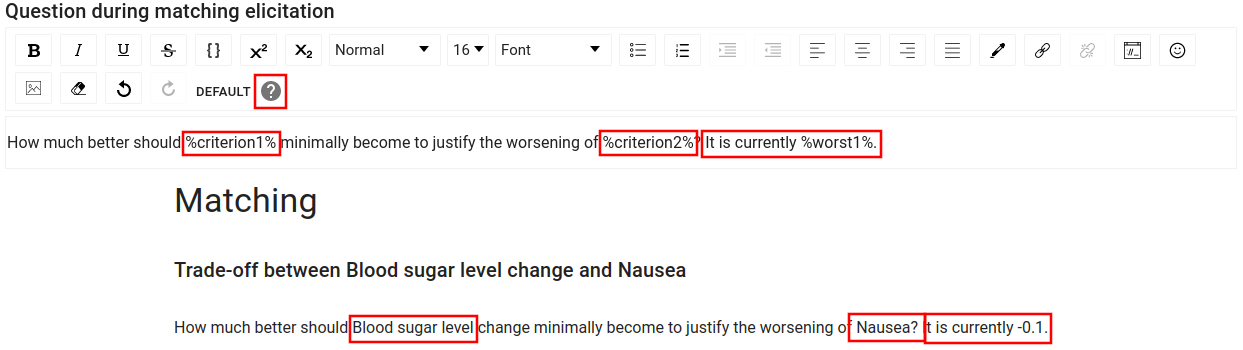
\includegraphics[width=\textwidth]{fig/templateStrings.png}
	\captionof{figure}{Modifying a question with templates, during and after editing. Note the explanation text which is toggled using the '?' button. Templates are substituted by their corresponding values when shown to the surveyee.}
	\label{fig:templateEditing}
	\par
}

\noindent \leftpointright \, Make any further changes you wish and continue your test run. Any changes you made have been saved, as you will see after ending the test run.
\newline

\noindent \leftpointright \, Enter any text as your identifier, and proceed. Select the most important criterion, and proceed again. Now you are presented with a matching trade-off scenario. \newline



\noindent \leftpointright \, Proceed through the elicitation process until the final screen. Note that again you can edit this text.
\newline

\noindent \leftpointright \, Assuming that the test run proceeded to your satisfaction, you are now ready to publish your survey. Proceed to the 'Publish' tab and click the 'Publish survey' button. This is also where you can close the survey for responses once its projected running time has ended. After publishing your survey, it will be available to anyone at the displayed URL.
\newline

\noindent \faLightbulbO \, If you are logged into the ADDIS/MCDA system, going to a survey URL that you own will let you manage it as you have been doing. Other users will see only the elicitation survey, as you will verify in the next step.
\newline

\subsection*{Collecting and analysing survey responses}

\noindent \leftpointright \, Open a new private browser window and go to the survey URL. You should be presented with the welcome screen as you configured it.
\newline

\noindent \leftpointright \, We need some completed surveys for the next step, so in this new window complete the survey at least three times, with different preferences.
\newline

\noindent \leftpointright \, Close the private window and return to the main survey interface. Click on the 'Responses' tab, and you should see the responses you provided in a table, with an overview of their preferences  (Fig.~\ref{fig:survey_responses})
\newline

{	
	\centering
	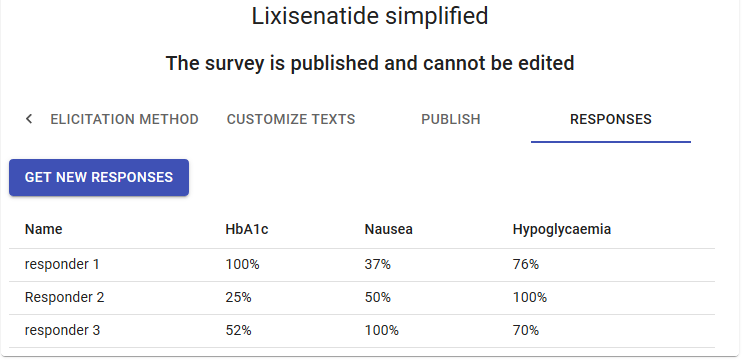
\includegraphics[width=\textwidth]{fig/surveyResponses.png}
	\captionof{figure}{The survey response table.}
	\label{fig:survey_responses}
	\par
}


\noindent \leftpointright \, Return to the main ADDIS/MCDA application, and refresh the page. The 'Survey results' tab should now be available if you have selected the problem for which you created the survey. Click on this tab.
\newline

\noindent \faGraduationCap \, The ADDIS/MCDA survey response analysis is based on our SMAA (Stochastic Multicriteria Acceptability Analysis) interface, but instead of sampling stochastically from the possibility space of the constraints given by the measurements and preferences, each survey response is treated as a sample. Therefore, the rank acceptabilities now show the distribution of preferences in the surveyed population, i.e. which proportion of the population would assign each rank to each alternative. Similarly, the weights shown for each criterion are sampled from distributions which are constrained by the survey responses.
\newline

\noindent \leftpointright \, Take a moment to examine the interface. We assume you are already familiar with the SMAA tab. The main difference here is the 'Survey responses' table which shows an overview of which responses are included in the analysis, similar to the responses tab in the survey tool. Note the distribution of the rank acceptabilities, and see whether you can deduce which responses are responsible for which ranks.
\newline

\noindent \leftpointright \, Click the + button next to the selected 'Everything' aggregated analysis at the top of the page (Fig.~\ref{fig:survey_response_analysis}). Add a new aggregated analysis where you have excluded at least one of your scenario responses.
\newline

{	
	\centering
	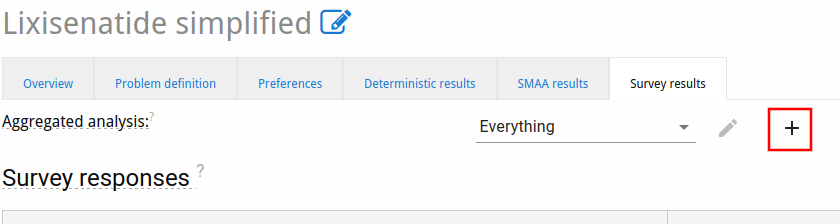
\includegraphics[width=\textwidth]{fig/surveyResponseAnalysis.png}
	\captionof{figure}{Survey analysis creation button.}
	\label{fig:survey_response_analysis}
	\par
}

\noindent \leftpointright \, Switch back and forth between the automatically-generated 'Everything' aggregated analysis and the new reduced one you just created, and note any differences. Can you explain them based on the excluded survey response?

\subsection*{Final words}
This tutorial showed how to create durveys starting from an analysable effects table. It also demonstrated how to customise the survey, and preview the consequences of any changes. Finally, it showed how to obtain an overview of the survey responses and analyse them in ADDIS/MCDA.

\end{sidebar*}
\end{document}
